% !TEX root= ../main.tex
\section{Unary NAND-clauses in graph theories}
\label{sec:Unary NAND-clauses in graph theories}
We will to use the fact that some binary NAND-clauses are not binary-derivable to show that some \textit{unary} NAND-clauses are not binary-derivable.

We use our graph from Figure~\ref{fig:open_door} to make the following, bigger graph:\par
\begin{figure}[!h]
  \centering
  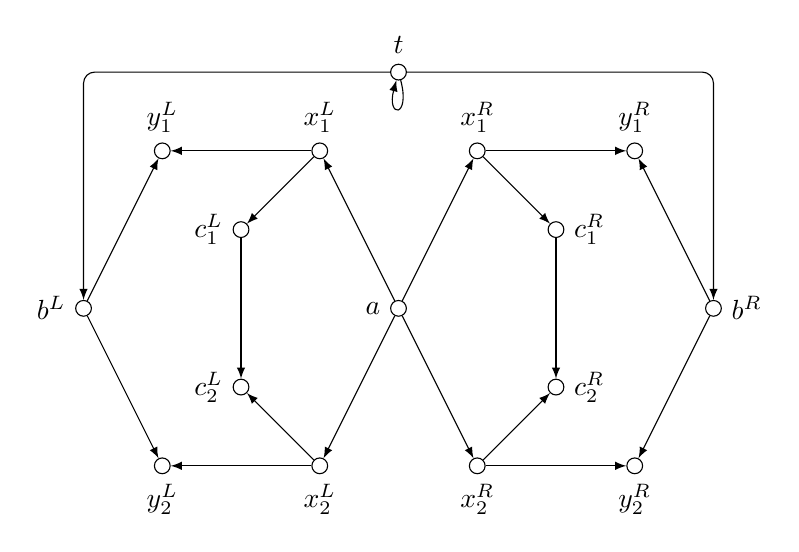
\begin{tikzpicture}
    [
    point/.style={circle,draw,inner sep=0pt,minimum size=2mm}
    ]
    \node (t) at (4,5) [point,label=above:$t$] {};
    \node (a) at (4,2) [point,label=left:$a$] {};
    \node (lx1) at (3,4) [point,label=above:$x^L_1$] {};
    \node (lx2) at (3,0) [point,label=below:$x^L_2$] {};
    \node (lb) at (0,2) [point,label=left:$b^L$] {};
    \node (ly1) at (1,4) [point,label=above:$y^L_1$] {};
    \node (ly2) at (1,0) [point,label=below:$y^L_2$] {};
    \node (lc1) at (2,3) [point,label=left:$c^L_1$] {};
    \node (lc2) at (2,1) [point,label=left:$c^L_2$] {};
    \draw [-latex] (a) to (lx1);
    \draw [-latex] (a) to (lx2);
    \draw [-latex] (lb) to (ly1);
    \draw [-latex] (lb) to (ly2);
    \draw [-latex] (lx1) to (ly1);
    \draw [-latex] (lx1) to (lc1);
    \draw [-latex] (lx2) to (ly2);
    \draw [-latex] (lx2) to (lc2);
    \draw [-latex] (lc1) to (lc2);
    \node (rx1) at (5,4) [point,label=above:$x^R_1$] {};
    \node (rx2) at (5,0) [point,label=below:$x^R_2$] {};
    \node (rb) at (8,2) [point,label=right:$b^R$] {};
    \node (ry1) at (7,4) [point,label=above:$y^R_1$] {};
    \node (ry2) at (7,0) [point,label=below:$y^R_2$] {};
    \node (rc1) at (6,3) [point,label=right:$c^R_1$] {};
    \node (rc2) at (6,1) [point,label=right:$c^R_2$] {};
    \draw [-latex] (a) to (rx1);
    \draw [-latex] (a) to (rx2);
    \draw [-latex] (rb) to (ry1);
    \draw [-latex] (rb) to (ry2);
    \draw [-latex] (rx1) to (ry1);
    \draw [-latex] (rx1) to (rc1);
    \draw [-latex] (rx2) to (ry2);
    \draw [-latex] (rx2) to (rc2);
    \draw [-latex] (rc1) to (rc2);

    \draw [-latex, rounded corners] (t) -| (lb);
    \draw [-latex, rounded corners] (t) -| (rb);
    \draw [-latex, loop below] (t) to (t);
  \end{tikzpicture}
  \caption{}
  \label{fig:double_open_door}
\end{figure}
\FloatBarrier
The above graph contains two copies of the graph from Figure~\ref{fig:open_door}, only connected by their shared vertex $a$ and the vertex $t$ that has both $b^L$ and $b^R$ in its neighborhood.
We will refer to the two copies as the left component and the right component, with $a$ being in both and $t$ being in none.

The rest of this section will show that the unary NAND-clause $\ol{a}$ is provable, but not binary derivable.

